\chapter{Grundlagen}

Zunächst stellen wir die verwendete Terminologie und relevante Konzepte bzw. Phänomene dar.

\section{Eingabe}
Unsere Eingabe sei durch eine $n$-elementige Zeichenfolge $S=e_1...e_n$ über dem beschränkten numerischen Alphabet $\Sigma$ mit $e_i\in \Sigma$ $\forall i=1,...,n$ gegeben. Für jede
beliebige Zeichenfolge $S$ wird mit $|S|$ dessen Länge, hier $n$, bezeichnet. Der Ausdruck $S[i..j]\in \Sigma^{j-i+1}$ mit $1\leq i\leq j\leq n$ beschreibt die Teilfolge $e_i...e_j$,
wobei im Falle, dass $i=j$ ist, das einzelne Zeichen $e_i$ referenziert wird. Alternativ kann ein einzelnes Zeichen $e_i$ auch durch $S[i]$ referenziert werden. Eine Teilfolge 
der Form $S[1..k]$ mit $1\leq k\leq n$ wird als Präfix von $S$ bezeichnet. Im Gegensatz dazu wird eine Teilfolge der Form $S[k..n]$ als Suffix von $S$ bezeichnet. Für zwei Teilfolgen
$S_1$ und $S_2$ beschreibt der Ausdruck $S_1+S_2$ die Konkatenation der beiden Teilfolgen.

\section{Ausgabe $\rightarrow$ Faktorisierung}
Ein charakteristisches Merkmal der Familie der Lempel-Ziv-Kompressionsverfahren ist die Repräsentation der Ausgabe in Form einer Faktorisierung. Für eine Eingabe $S=e_1...e_n$ 
wird eine Faktorisierung $F=f_1...f_z$ mit $z\leq n$ derart erzeugt, dass die Eingabe $S$ durch die Faktorisierung in eine equivalente Folge von nichtleeren Teilfolgen zerlegt wird. Dabei
ist jeder Faktor $f_i$ mit $1\leq i\leq z$ als nichtleerer Präfix von $S[|f_1...f_i-1|+1..n]$ definiert, der bereits in $S[1..|f_1...f_i|]$ vorkommt, oder als einzelnes Zeichen.
Die im Folgenden betrachteten Algorithmen können speziell der Klasse der LZ77-Kompressionsverfahren zugeordnet werden, dessen Faktoren im Schema des Lempel-Ziv-Storer-Szymanski
\cite{lzss} repräsentiert werden sollen. 

\begin{equation} \label{eq:faktor}
    F = f_1...f_z \text{ mit } f_i = \begin{cases} (Length, Position) & \text{falls Referenz} \\ (0, Zeichen) & \text{sonst} \end{cases}
\end{equation}

Zur Darstellung von Referenzen wird das Tupel aus der Position des vorherigen Vorkommens und der Länge des Faktors genutzt. Einzelne Zeichen können wiederum durch das Tupel aus dem Platzhalter 0 und dem
entsprechenden Zeichen dargestellt werden. Das in \ref{eq:faktor} definierte Format beschreibt die gewünschte Ausgabe der im Folgenden betrachteten Algorithmen.

\section{Kompression} \label{comp}

\subsection{Verlustfreie Kompression}
Der Prozess der Kompression überführt eine Repräsentation einer finiten Datenmenge in eine möglichst kompaktere Form. Eine verlustfreie Kompression ist gegeben, falls die Abbildung
zwischen der ursprünglichen und komprimierten Repräsentation bijektiv ist. Die Korrektheit einer verlustfreien Kompression kann daher durch die Angabe einer Dekompressionsfunktion 
nachgewiesen werden. Ist diese Vorraussetzung nicht gegeben, so handelt es sich um eine verlustbehaftete Kompression, da eine Rekonstruktion der ursprünglichen Datenmenge nicht 
garantiert werden kann.

\subsection{Dekompression}
Die Dekompression beschreibt den Umkehrprozess der Kompression und erlaubt im Falle eine verlustfreien Kompression die Rekonstruktion der ursprünglichen Datenfolge. Im Falle von 
Verfahren der LZ77-Familie, kann die Dekompression durch die folgende Abbildung definiert werden, 
\begin{equation}
    DECOMP_{LZ77}: F(1..z) \rightarrow S(1..n).
\end{equation}

\begin{algorithm} [ht]
\centering
\caption{DECOMP$_{LZ77}$} \label{alg:decomp}
\algorithmicrequire $F=f_1...f_z$
\algorithmicensure $S=e_1...e_n$
\begin{algorithmic}
    \STATE $S \gets \emptyset$
    \FOR{$i=1$ to $z$}
        \STATE (len, ref) $\gets f_i$
        \IF{len = 0} 
            \STATE $S \gets S + ref$
        \ELSE
            \FOR{$j=0$ to $len-1$}
                \STATE $S \gets S + S[ref + j]$
            \ENDFOR
        \ENDIF
    \ENDFOR
    \RETURN $S$
\end{algorithmic}
\end{algorithm}

Der dargestellte Algorithmus \ref{alg:decomp} beschreibt eine mögliche Implementierung der Dekompression für eine Faktorisierung $F=f_1...f_z$ zu der Eingabe $S=e_1...e_n$.
Der beschriebene Algorithmus iteriert durch alle Faktoren und fügt die referenzierten Zeichen einzeln in die Ausgabe $S$ ein. Damit kann die Laufzeit des Algorithmus auf $O(n)$
geschätzt werden.

\subsection{String-Matching $\rightarrow$ Rabin-Karp}
Im Rahmen des approximativen Algorithmus, welcher in dieser Arbeit beschrieben wird, werden Vergleiche von Zeichenfolgen mithilfe des Rabin-Karp-Fingerprints(RFP)\cite{ApproxLZ77}
durchgeführt. Sei
$p\in \mathbb{P}$ eine Primzahl und $b\in \mathbb{N}$ eine Basis, so kann der RFP einer Zeichenfolge $S$ der Länge $n$ durch den Ausdruck
\begin{equation}
    \begin{split}
    RFP(S) &= \sum_{i=1}^{n} S[i]b^{n-i} \mod p \\
    &\in \{0,...,p-1\}
    \end{split}
\end{equation}
berechnet werden. Hierbei wird eine Zeichenfolge beliebiger Länge in eine Zahl aus dem Intervall $[0,p-1]$ abgebildet. Der RFP erlaubt es, die Gleichheit zweier Zeichenfolgen zu widerlegen
im Falle von unterschiedlichen Werten. Im Falle von gleichen RFPs, kann die Gleichheit der Zeichenfolgen jedoch nicht garantiert werden. Die Wahrscheinlichkeit einer Kollision 
dieser Art bei Zeichenfolgen gleicher Größe ist jedoch beschränkt und praktisch gering\cite{ApproxLZ77}. Insbesondere kann die Wahrscheinlichkeit durch die passende Wahl von $p$ und $b$ 
minimiert werden.

Rabin-Karp-Fingerprints erlauben verschiedene Operationen auf Zeichenfolgen, die im Rahmen der approximativen LZ77-Faktorisierung effizient genutzt werden können. Zum Einen kann ein
beschränktes Fenster $S_{W} = S(j..j+w)$ der Länge $w<n$ leicht verschoben werden. Sei $RFP(S_{W})$ der Fingerabdruck des Fensters, so kann der Fingerprint durch die Verschiebung um 
ein Zeichen nach rechts durch den Ausdruck,
\begin{equation} \label{eq:shift}
    RFP(S(j+1..j+w+1)) = (RFP(S_W) - S[j]b^{w-1})b + S[j+w+1] \mod p,
\end{equation}
beschrieben werden. Desweiteren seien zwei Teilfolgen $S_1$ und $S_2$ der gleichen Länge $n$ gegeben. Der RFP der Konkatenation,$S_1+S_2$, der beiden Teilfolgen kann durch den Ausdruck,
\begin{equation} \label{eq:concat}
    RFP(S_1 + S_2) = (RFP(S_1)b^n + RFP(S_2)) \mod p,
\end{equation}
berechnet werden. Analog zur Konkatenation von Zeichenfolgen ist die Operation \ref{eq:concat} ebenfalls assoziativ, jedoch nicht kommutativ.

\subsection{Verlustbehaftete Kompression}
Im Rahmen dieser Arbeit werden wir einen Approximationsalgorithmus betrachten, der aufgrund der verwendeten RFP-Technik für Vergleiche von Zeichenfolgen eine fehlerhafte Faktorisierung mit 
einer beschränkten Wahrscheinlichkeit erzeugen kann. Die Korrektheit der Dekompression kann intern und extern durch explizite Vergleiche der Zeichenfolgen erkannt werden. Da der
Kompressionsprozess in diesem Fall mit anderen Parametern wiederholt werden kann, können wir einen verlustfreien Las-Vegas-Algorithmus konstruieren.

\begin{figure}
    \centering
    \caption{Konstruktion eines verlustfreien Las-Vegas-Algorithmus durch Wiederholung des verlustbehafteten Kompressionsprozesses}
    \label{fig:lasvegas}
    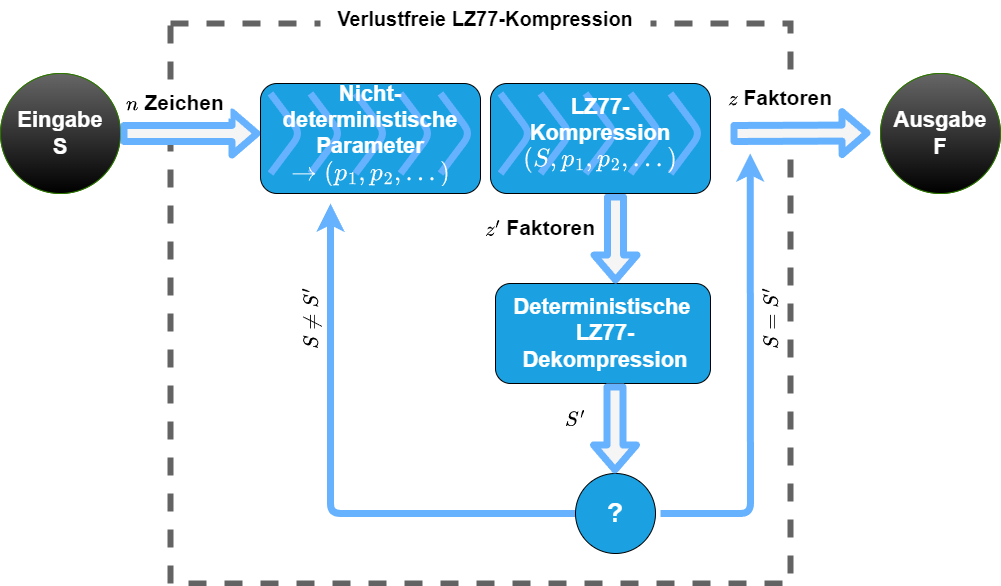
\includegraphics[scale=0.25]{Images/lasvegas_algorithm.png}
\end{figure}

In Abbildung \ref{fig:lasvegas} wird eine Regelsteuerung illustriert. Der Algorithmus wird solange wiederholt, bis eine korrekte Faktorisierung erzeugt wurde. Dass die
Anzahl der Wiederholungen beschränkt ist, werden wir in der Analyse des Approximationsalgorithmus und der praktischen Evaluation zeigen.

\subsection{Binäre (De-)Kodierung}
Die Kodierung $K_{IN}: \Sigma^* \rightarrow \{0,1\}^*$ überführt unsere Eingabe aus dem Alphabet $\Sigma$ in eine binäre Repräsentation.
Die Umkehrabbildung $K^{-1}_{IN}: \{0,1\}^* \rightarrow \Sigma^*$ definiert die Dekodierung und überführt eine binäre Repräsentation in eine Zeichenfolge
aus dem Alphabet $\Sigma$. Im Rahmen dieser Arbeit gehen wir davon aus, dass unsere Eingabe $S$ über dem Alphabet $\Sigma=\{1,...,255\}$ erzeugt wurde und 
jedes Zeichen durch 8 Bits, oder 1 Byte, dargestellt wird. Für die Länge, $|S|_{Bin}$, der binären Repräsentation folgt,
\begin{equation}
    |S|_{Bin} = |K_{IN}(S)| = 8*|S|.
\end{equation}

Die eingelesene Eingabefolge wird durch den Kompressionsalgorithmus in die Faktorfolge $F=f_1...f_z$ überführt. Die bijektive Abbildung $K_{OUT}: F \rightarrow \{0,1\}^*$
definiert die Kodierung der Faktoren in eine binäre Repräsentation. Analog dazu wird die Dekodierung $K^{-1}_{OUT}: \{0,1\}^* \rightarrow F$ definiert. Im Gegensatz zur Eingabe, 
werden wir keine Kodierung bzw. Dekodierung der Faktoren vorgeben, da diese durch den Kompressionsalgorithmus nicht beschränkt wird. Für eine beliebige lineare Kodierung $K_{OUT}$ ergibt 
sich die binäre Ausgabegröße $|F|_{Bin}$ durch
\begin{equation}
    |F|_{Bin} = \sum_{i=1}^{z} |K(f_i)|.
\end{equation}

\subsection{Metriken}
Die Qualität einer Kompression kann durch verschiedene Metriken quantifiziert werden. Zum Einen beschreibt die Kompressionsrate $CR$ den Grad der Kompression und ist durch den
Ausdruck, 
\begin{equation}
    CR = \frac{|F|_{Bin}}{|S|_{Bin}}
\end{equation}
, definiert.
Da die Kodierung der Faktoren nicht eindeutig aus der Wahl des Kompressionsalgorithmus eingegrenzt wird, ist stattdessen die Anzahl der erzeugten Faktoren ein
weiteres geeignetes Gütemaß. Für die Eingabe $S$ der Länge n und der Ausgabe $f_1...f_z$ sei die Faktorrate durch
\begin{equation}
    FR = \frac{z}{n}
\end{equation}
gegeben. In beiden Fällen wird ein niedriger Wert bevorzugt, da dieser auf eine bessere Extraktion von Redundanzen hinweist.

\section{Parallelität}
Das Ziel dieser Arbeit ist die Entwicklung und Evaluation eines parallel Kompressionsalgorithmus. Im Folgenden definieren wir die Rahmenbedingungen und Konzepte der Parallelität.

\subsection{Shared-Memory-Modell}
Unser Algorithmus agiert auf einem Shared-Memory-Modell mit $P$ Ausführungseinheiten, welches im Gegensatz zum Distributed-Memory-Modell allen beteiligten 
Ausführungseinheiten bzw. Prozessoren einen gemeinsamen Zugriff auf den Speicher ermöglicht. Im Rahmen der parallelen Programmierung muss der simultane Lese- bzw. Schreibzugriff auf
Speicherbereiche synchronisiert werden, um Konflikte zu vermeiden. Die Konsequenz einer mangelnden oder ineffizienten Synchronisation können Inkonsistenzen in der Korrektheit und
Performanz des Algorithmus sein. In der Praxis manifestieren sich diese Probleme beispielsweise in Form von Data-Races oder False-Sharing.\cite{parallelcomputing}
Unser parallel modellierte Algorithmus muss explizit seine Korrektheit bewahren mit dem Ziel einer möglichst hohen Beschleunigung der Laufzeit.

\subsection{Metriken}
Das Ziel der Parallelisierung eines Algorithmus liegt hauptsächlich in einer Verbesserung der Laufzeit, insbesondere unter Berücksichtigung der bereits beschriebenen Ressourcenkonflikten. 
Die zeitliche Beschleunigung der Laufzeit kann durch den Speedup $SP$ bemessen werden. Für eine Eingabe $S$ der Länge $n$ brauche ein sequenzieller Durchlauf $T(n, p=1)$ Zeit, während ein 
paralleler Algorithmus mit $P$ Prozessoren $T(n,p=P)$ an Zeit benötigt. Der Speedup ist dabei definiert durch
\begin{equation}
    SP(n,P) = \frac{T(n,1)}{T(n,P)}.
\end{equation}
Ein idealer Speedup ist gegeben durch $SP(n,P)=P$. Verschiedene Effekte im Rahmen des Speicherzugriffs, der Synchronisation und der Kommunikation über mehrere Prozessoren können jedoch
die Effizienz der Parallelisierung stark beeinträchtigen. Insbesondere können sequenzielle Abschnitte im Algorithmus aufgrund des Amdahl'schen Gesetzes\cite{amdahl} eine obere Schranke 
für den Speedup setzen.

